\documentclass[tikz, border=10pt]{standalone}

\usepackage{tikz}
\usepackage{pgfmath}

\begin{document}
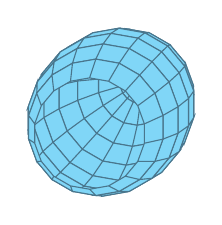
\begin{tikzpicture}
    \pgfsetfillcolor{cyan!50}
    \pgfsetstrokecolor{cyan!50!black}
    \foreach \latitude in {-90, -75, ..., 30}{
        \foreach \longitude in {0, 20, ..., 360}{
            \pgfpathmoveto{\pgfpointspherical{\longitude}{\latitude}{1}}
            \pgfpathlineto{\pgfpointspherical{\longitude+20}{\latitude}{1}}
            \pgfpathlineto{\pgfpointspherical{\longitude+20}{\latitude+15}{1}}
            \pgfpathlineto{\pgfpointspherical{\longitude}{\latitude+15}{1}}
            \pgfpathclose
        }
        \pgfusepath{stroke, fill}
    }
\end{tikzpicture}
\end{document}